
%% IMEJ-Apr18.tex
%% V1.0
%%
%% This is a template file demonstrating the use of IMEJ.cls
%% For support, please see https://marineenergyjournal.org
%%
%%
%% It is based on the IEEE transactions journal paper template 
%% by Michael Shell - see http://www.michaelshell.org/
%% It is not endorsed by any person or organization other than IMEJ

%%*************************************************************************
%% Legal Notice:
%% This code is offered as-is without any warranty either expressed or
%% implied; without even the implied warranty of MERCHANTABILITY or
%% FITNESS FOR A PARTICULAR PURPOSE! 
%% User assumes all risk.
%% In no event shall any contributor to this code be liable for
%% any damages or losses, including, but not limited to, incidental,
%% consequential, or any other damages, resulting from the use or misuse
%% of any information contained here.
%%
%% All comments are the opinions of their respective authors and are not
%% necessarily endorsed by any organization.
%%
%% This work is distributed under the LaTeX Project Public License (LPPL)
%% ( http://www.latex-project.org/ ) version 1.3, and may be freely used,
%% distributed and modified. A copy of the LPPL, version 1.3, is included
%% in the base LaTeX documentation of all distributions of LaTeX released
%% 2003/12/01 or later.
%% Retain all contribution notices and credits.
%% ** Modified files should be clearly indicated as such, including  **
%% ** renaming them and changing author support contact information. **
%%*************************************************************************



\documentclass[10pt,journal,a4paper,twoside]{./IMEJ}
%
% If IMEJ.cls has not been installed into the LaTeX system files,
% manually specify the path to it like:
% \documentclass[journal]{../sty/IMEJ}


% Some very useful LaTeX packages include:
% (uncomment the ones you want to load)


% *** CITATION PACKAGES ***
%
\usepackage{cite}
% cite.sty was written by Donald Arseneau
% V1.6 and later of IEEEtran pre-defines the format of the cite.sty package
% \cite{} output to follow that of the IEEE. Loading the cite package will
% result in citation numbers being automatically sorted and properly
% "compressed/ranged". e.g., [1], [9], [2], [7], [5], [6] without using
% cite.sty will become [1], [2], [5]--[7], [9] using cite.sty. cite.sty's
% \cite will automatically add leading space, if needed. Use cite.sty's
% noadjust option (cite.sty V3.8 and later) if you want to turn this off
% such as if a citation ever needs to be enclosed in parenthesis.
% cite.sty is already installed on most LaTeX systems. Be sure and use
% version 5.0 (2009-03-20) and later if using hyperref.sty.
% The latest version can be obtained at:
% http://www.ctan.org/pkg/cite
% The documentation is contained in the cite.sty file itself.


% *** GRAPHICS RELATED PACKAGES ***
%
\usepackage[pdftex]{graphicx}
% \usepackage[dvips]{graphicx}

% graphicx was written by David Carlisle and Sebastian Rahtz. It is
% required if you want graphics, photos, etc. graphicx.sty is already
% installed on most LaTeX systems. The latest version and documentation
% can be obtained at: 
% http://www.ctan.org/pkg/graphicx
% Another good source of documentation is "Using Imported Graphics in
% LaTeX2e" by Keith Reckdahl which can be found at:
% http://www.ctan.org/pkg/epslatex
%
% latex, and pdflatex in dvi mode, support graphics in encapsulated
% postscript (.eps) format. pdflatex in pdf mode supports graphics
% in .pdf, .jpeg, .png and .mps (metapost) formats. Users should ensure
% that all non-photo figures use a vector format (.eps, .pdf, .mps) and
% not a bitmapped formats (.jpeg, .png). The IEEE frowns on bitmapped formats
% which can result in "jaggedy"/blurry rendering of lines and letters as
% well as large increases in file sizes.
%
% You can find documentation about the pdfTeX application at:
% http://www.tug.org/applications/pdftex

% *** SYMBOL PACKAGES ***
\usepackage{textcomp}


% *** MATHS PACKAGES ***
\usepackage{amsmath}
% A popular package from the American Mathematical Society that provides
% many useful and powerful commands for dealing with mathematics.
%
% Note that the amsmath package sets \interdisplaylinepenalty to 10000
% thus preventing page breaks from occurring within multiline equations. Use:
\interdisplaylinepenalty=2500
% after loading amsmath to restore such page breaks as IEEEtran.cls normally
% does. amsmath.sty is already installed on most LaTeX systems. The latest
% version and documentation can be obtained at:
% http://www.ctan.org/pkg/amsmath


% *** SPECIALIZED LIST PACKAGES ***
%
%\usepackage{algorithm2e}


% *** ALIGNMENT PACKAGES ***
%
\usepackage{booktabs}
\usepackage{threeparttable}


% *** SUBFIGURE PACKAGES ***
\usepackage[caption=false,font=footnotesize]{subfig}

% subfig.sty, written by Steven Douglas Cochran, is the modern replacement
% for subfigure.sty, the latter of which is no longer maintained and is
% incompatible with some LaTeX packages including fixltx2e. However,
% subfig.sty requires and automatically loads Axel Sommerfeldt's caption.sty
% which will override IMEJ.cls' handling of captions and this will result
% in non-IEEE style figure/table captions. To prevent this problem, be sure
% and invoke subfig.sty's "caption=false" package option (available since
% subfig.sty version 1.3, 2005/06/28) as this is will preserve IEEEtran.cls
% handling of captions.
%
% The latest version and documentation of subfig.sty can be obtained at:
% http://www.ctan.org/pkg/subfig


% *** FLOAT PACKAGES ***
%
%\usepackage{fixltx2e}
% fixltx2e, the successor to the earlier fix2col.sty, was written by
% Frank Mittelbach and David Carlisle. This package corrects a few problems
% in the LaTeX2e kernel, the most notable of which is that in current
% LaTeX2e releases, the ordering of single and double column floats is not
% guaranteed to be preserved. Thus, an unpatched LaTeX2e can allow a
% single column figure to be placed prior to an earlier double column
% figure.
% Be aware that LaTeX2e kernels dated 2015 and later have fixltx2e.sty's
% corrections already built into the system in which case a warning will
% be issued if an attempt is made to load fixltx2e.sty as it is no longer
% needed.
% The latest version and documentation can be found at:
% http://www.ctan.org/pkg/fixltx2e


%\usepackage{stfloats}
% stfloats.sty was written by Sigitas Tolusis. This package gives LaTeX2e
% the ability to do double column floats at the bottom of the page as well
% as the top. (e.g., "\begin{figure*}[!b]" is not normally possible in
% LaTeX2e). It also provides a command:
%\fnbelowfloat
% to enable the placement of footnotes below bottom floats (the standard
% LaTeX2e kernel puts them above bottom floats). This is an invasive package
% which rewrites many portions of the LaTeX2e float routines. It may not work
% with other packages that modify the LaTeX2e float routines. The latest
% version and documentation can be obtained at:
% http://www.ctan.org/pkg/stfloats
% Do not use the stfloats baselinefloat ability as the IEEE does not allow
% \baselineskip to stretch. Authors submitting work to the IEEE should note
% that the IEEE rarely uses double column equations and that authors should try
% to avoid such use. Do not be tempted to use the cuted.sty or midfloat.sty
% packages (also by Sigitas Tolusis) as the IEEE does not format its papers in
% such ways.
% Do not attempt to use stfloats with fixltx2e as they are incompatible.
% Instead, use Morten Hogholm'a dblfloatfix which combines the features
% of both fixltx2e and stfloats:
%
% \usepackage{dblfloatfix}
% The latest version can be found at:
% http://www.ctan.org/pkg/dblfloatfix




%\ifCLASSOPTIONcaptionsoff
%  \usepackage[nomarkers]{endfloat}
% \let\MYoriglatexcaption\caption
% \renewcommand{\caption}[2][\relax]{\MYoriglatexcaption[#2]{#2}}
%\fi
% endfloat.sty was written by James Darrell McCauley, Jeff Goldberg and 
% Axel Sommerfeldt. This package may be useful when used in conjunction with 
% IEEEtran.cls'  captionsoff option. Some IEEE journals/societies require that
% submissions have lists of figures/tables at the end of the paper and that
% figures/tables without any captions are placed on a page by themselves at
% the end of the document. If needed, the draftcls IEEEtran class option or
% \CLASSINPUTbaselinestretch interface can be used to increase the line
% spacing as well. Be sure and use the nomarkers option of endfloat to
% prevent endfloat from "marking" where the figures would have been placed
% in the text. The two hack lines of code above are a slight modification of
% that suggested by in the endfloat docs (section 8.4.1) to ensure that
% the full captions always appear in the list of figures/tables - even if
% the user used the short optional argument of \caption[]{}.
% IEEE papers do not typically make use of \caption[]'s optional argument,
% so this should not be an issue. A similar trick can be used to disable
% captions of packages such as subfig.sty that lack options to turn off
% the subcaptions:
% For subfig.sty:
% \let\MYorigsubfloat\subfloat
% \renewcommand{\subfloat}[2][\relax]{\MYorigsubfloat[]{#2}}
% However, the above trick will not work if both optional arguments of
% the \subfloat command are used. Furthermore, there needs to be a
% description of each subfigure *somewhere* and endfloat does not add
% subfigure captions to its list of figures. Thus, the best approach is to
% avoid the use of subfigure captions (many IEEE journals avoid them anyway)
% and instead reference/explain all the subfigures within the main caption.
% The latest version of endfloat.sty and its documentation can obtained at:
% http://www.ctan.org/pkg/endfloat
%
% The IEEEtran \ifCLASSOPTIONcaptionsoff conditional can also be used
% later in the document, say, to conditionally put the References on a 
% page by themselves.


% *** PDF, URL AND HYPERLINK PACKAGES ***
%
\usepackage{url}
% url.sty was written by Donald Arseneau. It provides better support for
% handling and breaking URLs. url.sty is already installed on most LaTeX
% systems. The latest version and documentation can be obtained at:
% http://www.ctan.org/pkg/url
% Basically, \url{my_url_here}.


%========================================================================
% *** Do not adjust lengths that control margins, column widths, etc. ***
% *** Do not use packages that alter fonts (such as pslatex).         ***
%========================================================================


% correct bad hyphenation here
\hyphenation{infla-mmable}


\begin{document}
%
% Apply reference list directives (see example.bib and http://mirror.ox.ac.uk/sites/ctan.org/macros/latex/contrib/IEEEtran/bibtex/IEEEtran_bst_HOWTO.pdf)
\bstctlcite{IEEEexample:BSTcontrol}
%
% paper title
% Only the first word (and proper nouns) of titles are capitalized.
% Linebreaks \\ can be used within to get better formatting as desired.
% Do not put math or special symbols in the title.
\title{How to prepare your article for the International Marine Energy Journal\\(January 2018)}
%
%
% author names
% note positions of commas and nonbreaking spaces ( ~ ) LaTeX will not break
% a structure at a ~ so this keeps an author's name from being broken across
% two lines.
% use \thanks{} to gain access to the first footnote area
% a separate \thanks must be used for each paragraph as LaTeX2e's \thanks
% was not built to handle multiple paragraphs
%

\author{First A. Author,
        Second B. Author,
        and~Third C. Author% <-this % stops a space
\thanks{This paragraph of the first footnote will contain the date on which you submitted your paper for review and the open access licence (CC~BY). It will also contain support information, including sponsor and financial support acknowledgement. For example, `This work was supported in part by the EPSRC under grant...'}% <-this % stops a space
\thanks{The next few paragraphs should contain the authors’ current affiliations, including current address and e-mail. For example, F. A. Author is with the Energy and Environmental Sciences Branch Space and Naval Warfare Systems Center Pacific 53560 Hull Street San Diego, CA, 92152 U.S.A (e-mail: f.a.author@domain.tld).}% <-this % stops a space
\thanks{S. B. Author was at the French Research Institute for Exploitation of the Sea (IFREMER) Centre Manche---Mer du Nord, Boulogne sur Mer FR-62321, France. They are now at College of Engineering, Ocean University of China, Qingdao, China, 266100 (e-mail: s.b.author@domain.tld).}% <-this % stops a space
\thanks{T. C. Author is with Department of Physical Oceanography, CICESE, Carretera Ensenada-Tijuana 3918, Ensenada, Baja California, Mexico (e-mail: t.c.author@domain.tld).}
} % close \author


% note the % following the last \thanks - 
% these prevent an unwanted space from occurring between the last author name
% and the end of the author line. i.e., if you had this:
% 
% \author{....lastname \thanks{...} \thanks{...} }
%                     ^------------^------------^----Do not want these spaces!
%
% a space would be appended to the last name and could cause every name on that
% line to be shifted left slightly. This is one of those "LaTeX things". For
% instance, "\textbf{A} \textbf{B}" will typeset as "A B" not "AB". To get
% "AB" then you have to do: "\textbf{A}\textbf{B}"
% \thanks is no different in this regard, so shield the last } of each \thanks
% that ends a line with a % and do not let a space in before the next \thanks.



% The paper headers
\markboth{International Marine Energy Journal,~Vol.~VV, No.~NN, Month~Year}%
{First-author-surname \MakeLowercase{\textit{et al.}}: Paper-title}
% The only time the second header will appear is for the odd numbered pages
% after the title page when using the twoside option.
% 
% *** Note that you probably will NOT want to include the author's ***
% *** name in the headers of peer review papers.                   ***
% You can use \ifCLASSOPTIONpeerreview for conditional compilation here if
% you desire.




% If you want to put a publisher's ID mark on the page you can do it like
% this:
%\IMEJpubid{0000--0000/00\$00.00~\copyright~2015 IEEE}
% Remember, if you use this you must call \IMEJpubidadjcol in the second
% column for its text to clear the IEEEpubid mark.


% use for special paper notices
%\IMEJspecialpapernotice{(Invited Paper)}


% make the title area
\maketitle

% As a general rule, do not put math, special symbols or citations
% in the abstract or keywords.
\begin{abstract}
These instructions give you guidelines for preparing papers for IMEJ. Use this document as a template if you are using \LaTeX. Otherwise, use this document as an instruction set. The electronic file of your paper may be formatted further at IMEJ. Paper titles should have only the first letter and proper nouns in capitals, not each word capitalized or all uppercase. Avoid writing long formulas with subscripts in the title. Initials and surname are required. Put a space between authors’ initials. The abstract must be a concise yet comprehensive reflection of what is in your article. In particular, the abstract must be self-contained, without abbreviations, footnotes, or references. It should be a microcosm of the full article. The abstract must be between 150--250 words. Be sure that you adhere to these limits; otherwise, you will need to edit your abstract accordingly. The abstract must be written as one paragraph, and should not contain displayed mathematical equations or tabular material. The abstract should include three or four different keywords or phrases, as this will help readers to find it. Ensure that your abstract reads well and is grammatically correct.
\end{abstract}

% Note that keywords are not normally used for peerreview papers.
\begin{IMEJkeywords}
Enter at least three key words or phrases in alphabetical order, separated by commas.
\end{IMEJkeywords}


% For peer review papers, you can put extra information on the cover
% page as needed:
% \ifCLASSOPTIONpeerreview
% \begin{center} \bfseries EDICS Category: 3-BBND \end{center}
% \fi
%
% For peerreview papers, this IEEEtran command inserts a page break and
% creates the second title. It will be ignored for other modes.
\IMEJpeerreviewmaketitle


\section{Introduction}
% The very first letter is a 2 line initial drop letter followed
% by the rest of the first word in caps.
% Here we have a "T" for an initial drop letter
% and "HIS" in caps to complete the first word.
\IMEJPARstart{T}{his} document is a template for \LaTeX\ using IMEJ.cls version 1.0 and later. If you are reading a paper or PDF version of this document, please download the package, IMEJ-template-Jan18.zip, from the IMEJ web site at \url{marineenergyjournal.org} so you can use it to prepare your manuscript. If you would prefer to use \textit{LibreOffice Writer} or \textit{Microsoft Word}, download the appropriate template from the same web page. 
The style file IMEJ-template-Jan18.cls (included in the package) will adjust your fonts and line spacing. Do not change the font sizes or line spacing to squeeze more text into a limited number of pages. Use italics for emphasis; do not underline. 
Section and subsection headings should have only the first letter and proper nouns in capitals, not each word capitalized or all uppercase. The first word of the first section is capitalized, with the first letter as a `drop cap' spanning two lines.  Therefore you must have at least two lines in the paragraph with the drop letter.

\subsection{Abbreviations and acronyms}
Define abbreviations and acronyms the first time they are used in the text, even after they have already been defined in the abstract. Abbreviations such as IMEJ, 3D, and GIS do not have to be defined. Abbreviations that incorporate periods should not have spaces: write `C.N.R.S.,' not `C. N. R. S.' Do not use abbreviations in the title unless they are unavoidable.

% needed in second column of first page if using \IMEJpubid
%\IMEJpubidadjcol

\subsection{Other recommendations}
Use one space after periods and colons. Hyphenate complex modifiers: `cube-root-mean-cube.' Avoid dangling participles, such as, `Using (1), the power was calculated.' [It is not clear who or what used (1).] Write instead, `The potential was calculated by using (1),' or `Using (1), we calculated the potential.' 
Use a zero before decimal points: `0.25', not `.25.' Use `m$^3$,' not `cumec.' Indicate dimensions as `0.1 km\texttimes0.2 km,' not `0.1\texttimes0.2 km$^2$.' The abbreviation for `seconds' is `s,' not `sec.' Use `kW/m$^2$' or `kilowatts per square meter,' not `kilowatts/m$^2$.' When expressing a range of values, write `7 to 9' or `7--9,' not `7{\textasciitilde}9.'
A parenthetical statement at the end of a sentence is punctuated outside of the closing parenthesis (like this). (A parenthetical sentence is punctuated within the parentheses.) Avoid contractions; for example, write `do not' instead of `don’t.' The serial (or `Oxford') comma is not required in lists.
If you wish, you may write in the first person singular or plural and use the active voice (`I observed that ...' or `We observed that ...' instead of `It was observed that ...'). Remember to check spelling. If your first language is not English, please get an appropriate person to carefully proofread your paper.

\section{Mathematical formulae}
\subsection{Equations}
Number equations consecutively with equation numbers in parentheses flush with the right margin, as in (1). First use the equation editor to edit the equation. Then add an un-labelled caption, which must then be cut and paste into the final column. To make your equations more compact, you may use the solidus ( / ), the exp() function, or appropriate exponents. Use parentheses to avoid ambiguities in denominators.
Be sure that the symbols in your equation have been defined before the equation appears or immediately following. Italicize symbols (T might refer to temperature, but T is the unit tesla). Refer to `(1),' not `Eq.~(1)' or `equation~(1),' except at the beginning of a sentence: `Equation~(1) is ... .'

\section{Units}
Use SI (MKS) as primary units. Imperial units may be used as secondary units (in parentheses). An exception is when Imperial units are used as identifiers in trade, such as `3{\textonehalf}-in pipe.' Avoid combining SI and CGS units, such as flow in cm/s. This often leads to confusion because equations do not balance dimensionally. If you must use mixed units, clearly state the units for each quantity in an equation.

\section{Some common mistakes}
The word `data' is plural, not singular. A graph within a graph is an `inset,' not an `insert.' The word `alternatively' is preferred to the word `alternately' (unless you really mean something that alternates). Use the word `whereas' instead of `while' (unless you are referring to simultaneous events). Do not use the word `essentially' to mean `approximately' or `effectively.' Do not use the word `issue' as a euphemism for `problem.' 
Be aware of the different meanings of the homophones `affect' (usually a verb) and `effect' (usually a noun), `complement' and `compliment,' `discreet' and `discrete,' `principal' (e.g., `principal investigator') and `principle' (e.g., `principle of measurement'). Do not confuse `imply' and `infer.' 
Prefixes such as `non,' `sub,' `micro,' `multi,' and `ultra' are not independent words; they should be joined to the words they modify, usually without a hyphen. There is no period after the `et' in the Latin abbreviation `et~al.' (it is also not italicized). The abbreviation `i.e.,' means `that is,' and the abbreviation `e.g.,' means `for example' (these abbreviations are not italicized).
The suffix `-ize' is correct, both phonetically and etymologically, in both British and American English and there is no reason to use `-ise.' For further information, please see the relevant entry in the Oxford English Dictionary. 

\section{Guidelines for graphics preparation and submission}
\subsection{Types of graphics}
The following list outlines the different types of graphics published in IMEJ journals. They are categorized based on their construction, and use of colour or shades of grey:
\subsubsection{Colour/grey-scale figures}
Figures that are meant to appear in colour, or shades of black/grey. Such figures may include photographs, illustrations, multicolour graphs, and flowcharts.
\subsubsection{Line art figures}
Figures that are composed of only black lines and shapes. These figures should have no shades or half-tones of grey, only black and white.
\subsubsection{Tables}
Data charts which are typically black and white, but sometimes include colour.
\subsubsection{Multipart figures}
Figures compiled of more than one sub-figure presented side-by-side, or stacked. If a multipart figure is made up of multiple figure types (one part is line-art, and another is grey-scale or colour) the figure should meet the stricter guidelines.
\subsection{File formats for graphics}
Format and save your graphics using a suitable graphics processing program that will allow you to export  images as PostScript (PS), Encapsulated PostScript (.EPS), Tagged Image File Format (.TIFF), Portable Network Graphics (.PNG) or JPEG (.JPG) at suitable resolution (see below). It is strongly recommended that graphics be saved in PNG format rather than DOC, XLS, or PPT native formats. Doing so will protect your figures from common problems that occur when working on the files across multiple platforms. When submitting your final paper, your graphics should all be submitted individually in one of these formats along with the manuscript.
\subsection{Sizing of graphics}
Most charts, graphs, and tables are one column wide (86~mm) or page wide (178~mm). The maximum depth a graphic can be is 250~mm. When choosing the depth of a graphic, please allow space for a caption. Figures can be sized between column and page widths if the author chooses, however it is recommended that figures are not sized less than column width unless when necessary. 
IMEJ uses page size A4 with a column measurement of 86~mm. The column spacing is 6~mm. The left and right margins are 16~mm, top margin 22~mm (including header) and bottom margin 14~mm.  The header height is 10~mm.
\subsection{Raster graphics}
The proper resolution of your figures will depend on the type of figure it is as defined in the `Types of Figures' section. Photographs, and colour and grey-scale figures should be at least 300~dpi. Line art, including tables should be a minimum of 600~dpi. The JPEG format should only be used for photographs; PNG format should be used for diagrams as it preserves sharp boundaries.
\subsection{Vector graphics}
In order to preserve the integrity of figures across multiple computer platforms, we accept vector graphics in the following formats: .EPS/.PDF/.PS. All fonts must be embedded or text converted to outlines in order to achieve the best-quality results.
\subsection{Colour space}
The term colour space refers to the entire sum of colours that can be represented within the said medium. For our purposes, the three main colour spaces are: grey-scale, RGB (red/green/blue) and CMYK (cyan/magenta/yellow/black). RGB is generally used with on-screen graphics, whereas CMYK is used for printing purposes.
Colour figures should be generated all in RGB or all in CMYK colour space. grey-scale images should be submitted in grey-scale colour space. Line art may be provided in grey-scale OR bitmap colour space. Note that `bitmap colour space' and `bitmap file format' are not the same thing. When bitmap colour space is selected, .PNG or .TIFF are the recommended file formats.
\subsection{Accepted fonts within figures}
When preparing your graphics IMEJ suggests that you use of one of the following fonts: Palatino, Times New Roman, Helvetica, Arial, Cambria, and Symbol. If you are supplying EPS, PS, or PDF files all fonts must be embedded. Some fonts may only be native to your operating system; without the fonts embedded, parts of the graphic may be distorted or missing.
A safe option when finalizing your figures is to strip out the fonts before you save the files, creating `outline' type. This converts fonts to artwork what will appear uniformly on any screen.
\subsection{Using labels within figures}
\subsubsection{Figure axis labels}
Figure axis labels are often a source of confusion. Use words rather than symbols. As an example, write the quantity `Power,' or `Power $P$,' not just `$P$.' Put units in parentheses. Do not label axes only with units. As in \ref{fig_QP}, for example, write `Flow speed (m/s)' or `Flow speed (m$\cdot$s$^{-1}$),' not just `m/s.' Do not label axes with a ratio of quantities and units. For example, write `Pressure (Pa),' not `Pressure/Pa.' 
Multipliers can be especially confusing. Write `Pressure (kPa)' or `Pressure (10$^3$ Pa).' Do not write `Pressure Pa\texttimes1000' because the reader would not know whether the top axis label in \ref{fig_QP}\ meant 16000~Pa or 0.016~Pa. Figure labels should be legible, approximately 8 to 10 point type.
\subsubsection{Subfigure labels in multipart figures and tables}
Multipart figures should be combined and labelled before final submission. Labels should appear centred below each subfigure in 8 point Palatino font in the format of (a) (b) (c).
\subsection{File naming}
Figures (line artwork or photographs) should be named with the first author’s surname, followed by the number that represents the sequential location of this image in your article. For example, in author ``Smirnov's'' paper, the first three figures would be named smirnov1.tif, smirnov2.tif, and smirnov3.ps.
Tables should contain only the body of the table (not the caption) and should be named similarly to figures, except that ‘.t’ is inserted in-between the author’s name and the table number. For example, author ``Nguyen's'' first three tables would be named nguyen.t1.tif, nguyen.t2.ps, nguyen.t3.eps.
\subsection{Referencing a figure or table within your paper}
When referencing your figures and tables within your paper, use the abbreviation `Fig.' even at the beginning of a sentence. Do not abbreviate `Table.' Tables should be numbered with Roman numerals.
\subsection{Submitting your graphics}
Because IMEJ is run for and by the marine renewable energy community, without an external publisher and with only limited resources for graphical design, you are requested to position figures and tables at the top of each page, in the correct place in the document, as you would expect to see them in the final manuscript. In addition to submitting figures within your final manuscript, figures should be submitted individually, separate from the manuscript in one of the file formats listed above in section VI-C. Place figure captions below the figures; place table titles above the tables. Please do not include captions as part of the figures, or put them in `text boxes' linked to the figures. Also, do not place borders around the outside of your figures.
\subsection{Colour printing in IMEJ}
As the IMEJ is an online-only journal, an author can publish colour figures on IMEJ at no charge. However, authors may wish to bear in mind that readers will often print journal articles in monochrome.

% An example of a floating figure using the graphicx package.
% Note that \label must occur AFTER (or within) \caption.
% For figures, \caption should occur after the \includegraphics.
% Note that IEEEtran v1.7 and later has special internal code that
% is designed to preserve the operation of \label within \caption
% even when the captionsoff option is in effect. However, because
% of issues like this, it may be the safest practice to put all your
% \label just after \caption rather than within \caption{}.
%
% Reminder: the "draftcls" or "draftclsnofoot", not "draft", class
% option should be used if it is desired that the figures are to be
% displayed while in draft mode.
%
\begin{figure}[!t]
\centering
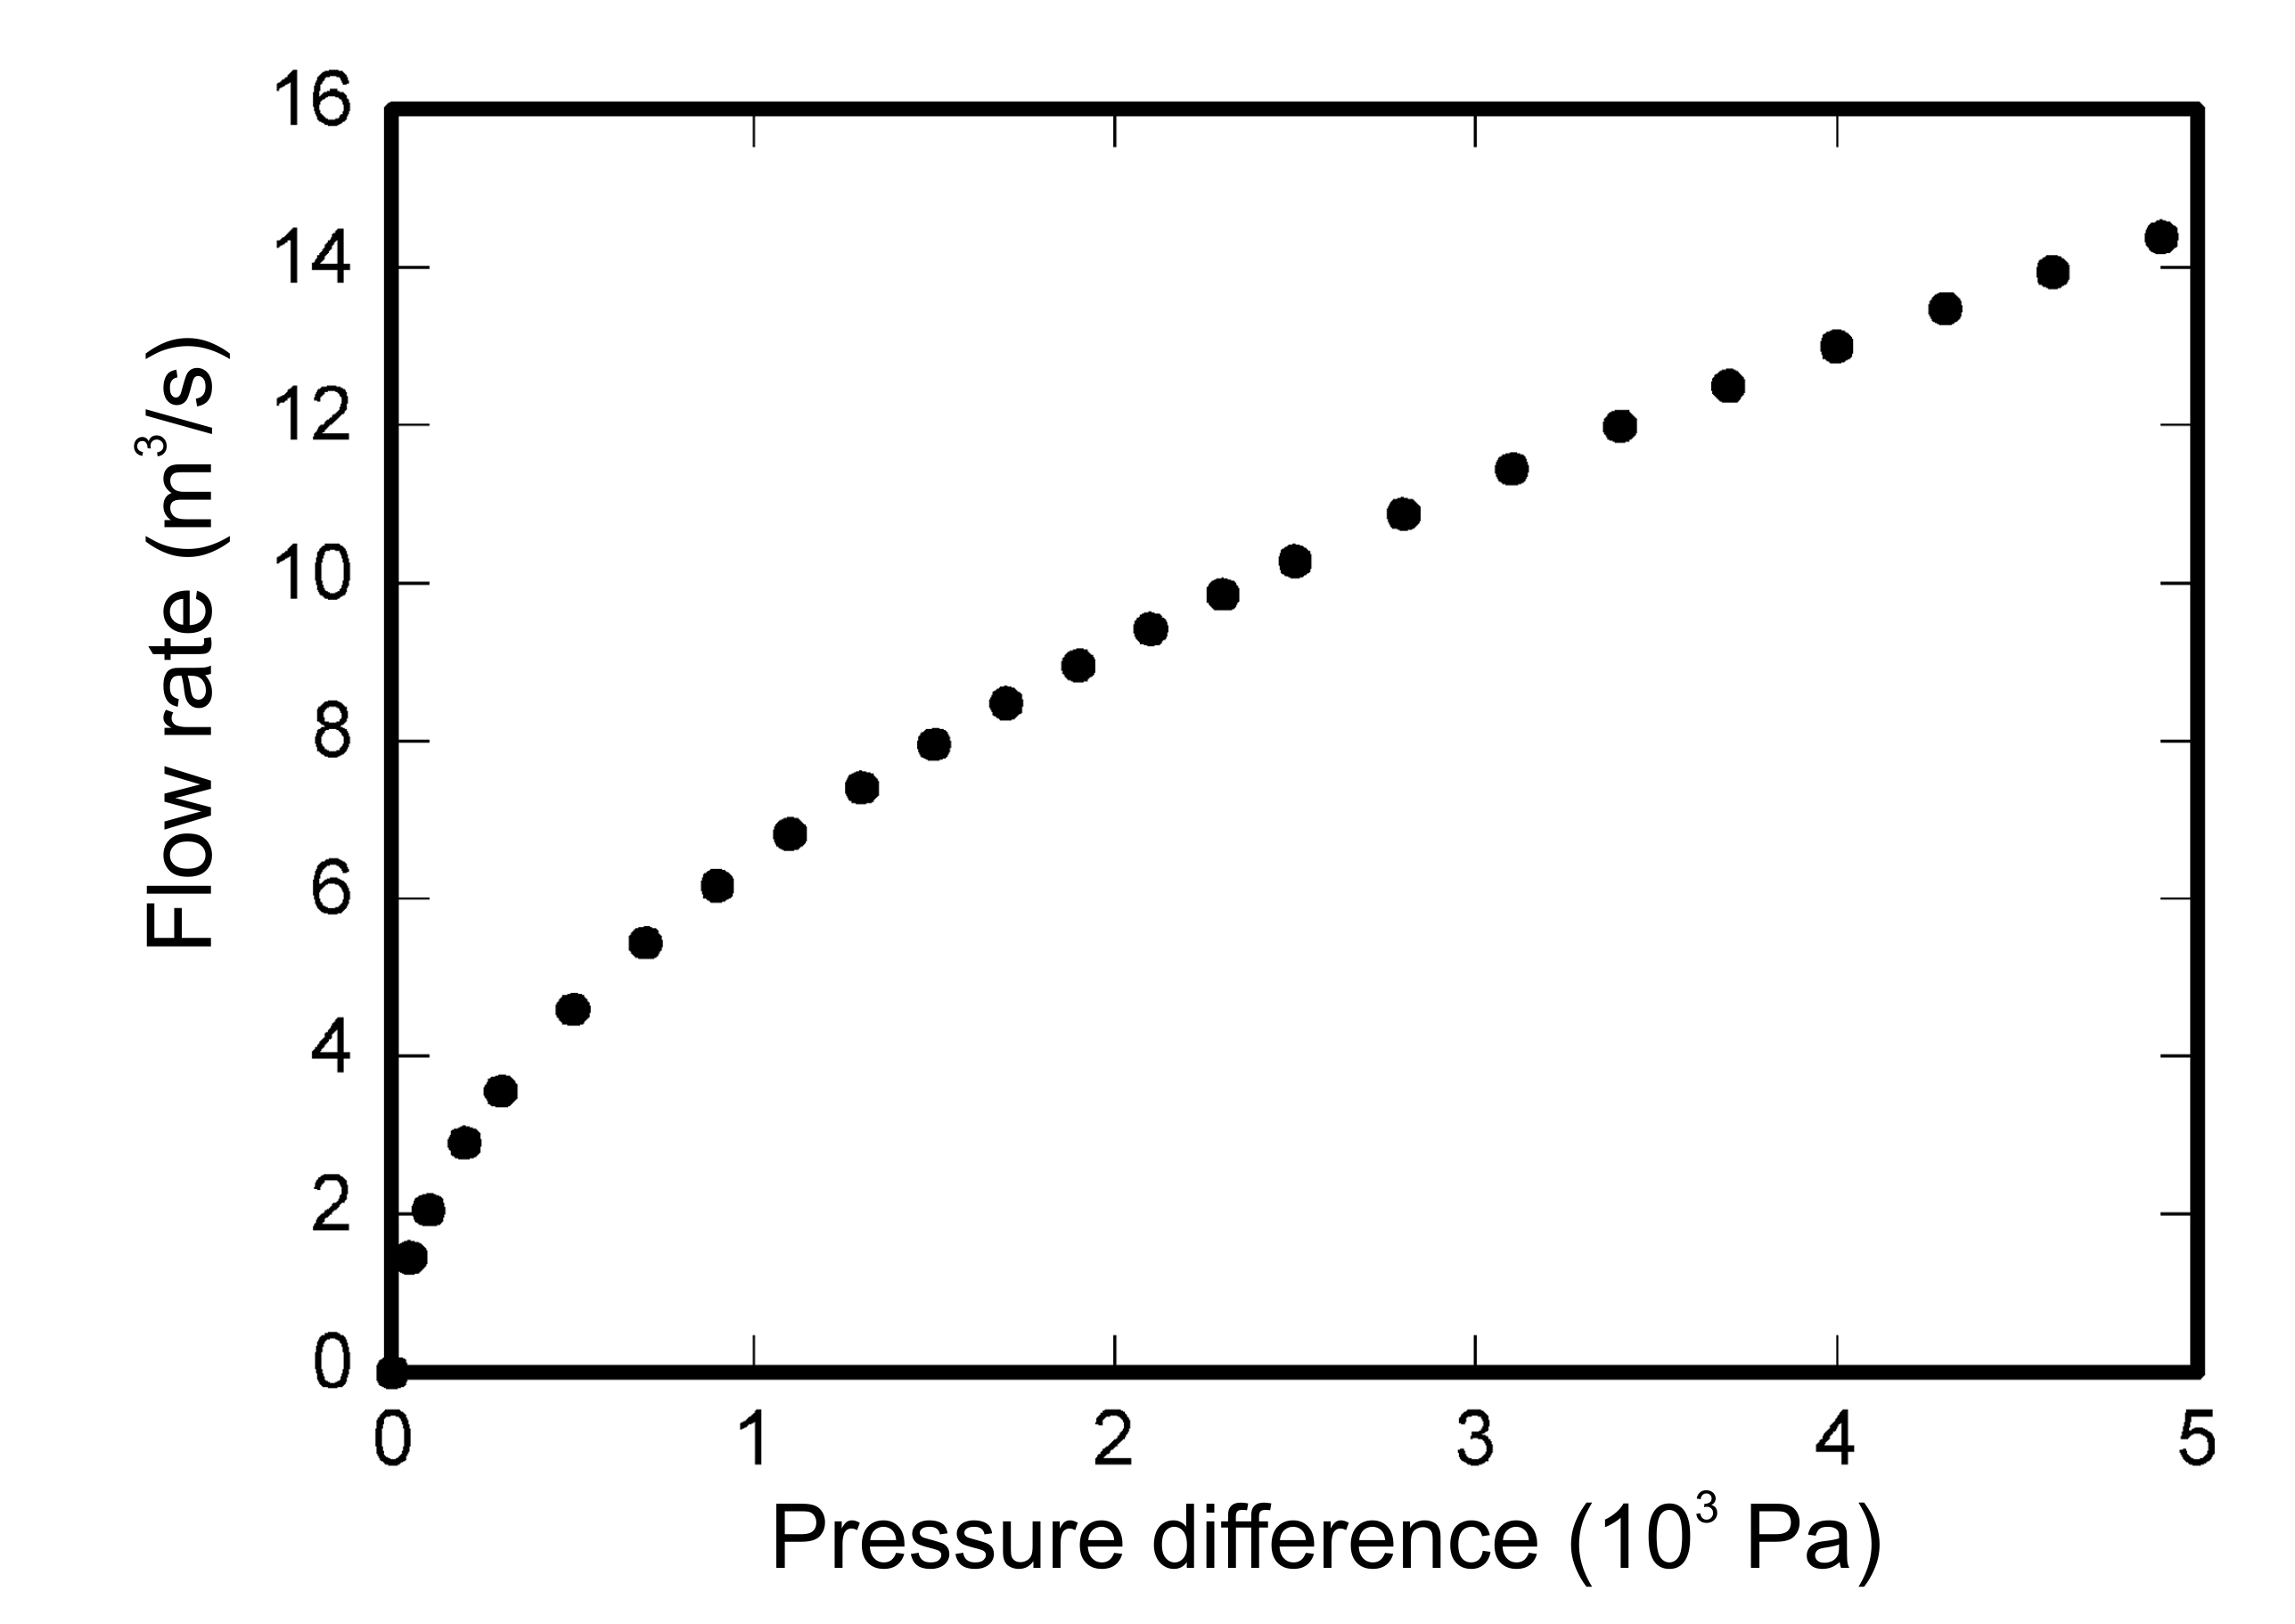
\includegraphics[width=86mm]{FlowVsPressure.png}
% where an .eps filename suffix will be assumed under latex, 
% and a .pdf suffix will be assumed for pdflatex; or what has been declared
% via \DeclareGraphicsExtensions.
\caption{Flow rate as a function of pressure difference. Note that ``Fig.'' is abbreviated. There is a period after the figure number, followed by two spaces. It is good practice to explain the significance of the figure in the caption.}
\label{fig_QP}
\end{figure}

% Note that the IEEE typically puts floats only at the top, even when this
% results in a large percentage of a column being occupied by floats.


% An example of a double column floating figure using two subfigures.
% (The subfig.sty package must be loaded for this to work.)
% The subfigure \label commands are set within each subfloat command,
% and the \label for the overall figure must come after \caption.
% \hfil is used as a separator to get equal spacing.
% Watch out that the combined width of all the subfigures on a 
% line do not exceed the text width or a line break will occur.
%
%\begin{figure*}[!t]
%\centering
%\subfloat[Case I]{[width=86mm]{FlowVsPressure.png}%
%\label{fig_first_case}}
%\hfil
%\subfloat[Case II]{[width=86mm]{FlowVsPressure.png}%
%\label{fig_second_case}}
%\caption{Flow rate as a function of pressure difference. Note that ``Fig.'' is abbreviated. There is a period after the figure number, followed by two spaces. It is good practice to explain the significance of the figure in the caption}
%\label{fig_QP2}
%\end{figure*}
%
% Note that often IEEE papers with subfigures do not employ subfigure
% captions (using the optional argument to \subfloat[]), but instead will
% reference/describe all of them (a), (b), etc., within the main caption.
% Be aware that for subfig.sty to generate the (a), (b), etc., subfigure
% labels, the optional argument to \subfloat must be present. If a
% subcaption is not desired, just leave its contents blank,
% e.g., \subfloat[].


% An example of a floating table. Note that the
% \caption command should come BEFORE the table and, similar to other titles in the document, only the first word and proper nouns should be in upper-case. Table text will default to \footnotesize as
% the IMEJ normally uses this smaller font for tables.
% The \label must come after \caption as always.
%
% Table generated by Excel2LaTeX (https://github.com/krlmlr/Excel2LaTeX)
% Other options for table generation from data: 
% - Gnumeric (https://help.gnome.org/users/gnumeric/)
% - R (https://cran.r-project.org/web/packages/xtable/index.html)
%
\begin{table}[!t]
\centering
\renewcommand{\arraystretch}{1.3}
\begin{threeparttable}
\caption{Example variables and units for marine renewable energy}
%
    \begin{tabular}{lll}
    \toprule
    Symbol & Quantity & Unit \\
    \midrule
    \textit{$U$} & Flow speed & 1 m/s = $0.51\dot{4}$ kn\tnote{a}\\
    \textit{$p$} & Pressure & Pa \\
    \textit{$\mu$} & Dynamic viscosity & Pa$\cdot$s \\
    \textit{$\nu$} & Kinematic viscosity & m$^2$/s \\
    \textit{$L$} & Distance & 1000 m = 1 km = $\frac{250}{463}$ nmi\tnote{a} \\
    \textit{$E$} & Energy & 1 kJ = $0.27\dot{7}$ kWh \\
    \textit{$a$} & Acceleration & m$\cdot$s$^{-2}$ \\
    \textit{$F$} & Force & N \\
    \textit{$P$} & Power & W \\
    \textit{$M$} & Mass  & 1000 kg = 1 t \\
    \textit{$Q$} & Flow rate & m$^3$/s \\
    \bottomrule
    \end{tabular}%
%
\begin{tablenotes}
\item Vertical lines in tables are deprecated. Statements that serve as captions for the entire table do not need footnote letters.
\item[a] The Admiralty measured mile and Admiralty knot should not be used to avoid confusion.
\end{tablenotes}
%
\end{threeparttable}
\label{tab:exUnits}%
\end{table}%
%
\section{References and footnotes}
\subsection{References}
In all references, the given name of the author or editor is abbreviated to the initial only and precedes the last name \cite{taylor1919}. Use them all; use et al. only if names are not given \cite{higgsBoson2015}. Abbreviate conference titles.  When referencing a patent, provide the day and the month of issue, or application. References should include enough information for the reader to find the original source. Do not combine references. There must be only one reference with each number \cite{falnes1991,castro1971,evans1987}. If there is a URL included with the print reference, it can be included at the end of the reference \cite{falnes1991,castro1971,evans1987,babarit2012}. 

Capitalize only the first word in a title, except for proper nouns and element symbols. For papers published in translation journals, please give the English citation first, followed by the original foreign-language citation.

\subsection{Footnotes}
It is recommended that footnotes be avoided (except for the unnumbered footnote with the receipt date on the first page). Instead, try to integrate the footnote information into the text.

\section{Submitting your paper for review}
\subsection{Review stage}
Contributions to the IMEJ may be submitted electronically on IMEJ’s online manuscript submission and peer-review system at \url{marineenergyjournal.org}.
First check if you have an existing account. If there is none, please register a new account. After logging in, select “Submissions” and then “New Submission.” 
Along with other information, you will be asked to confirm that the paper conforms to the publishing policy (see sections \ref{policy} and \ref{princi}). There are various steps to the submission process; you must complete all steps for a complete submission. You may compress large files prior to upload using \textit{7-Zip} or \textit{Gzip}. At the end of each step you must click “Save and Continue”; just uploading the paper is not sufficient. After the last step, you should see a confirmation that the submission is complete. You should also receive an e-mail confirmation. For inquiries regarding the submission of your paper, please contact \url{managing-editor@marineenergyjournal.org}. 

\subsection{No copyright transfer}
IMEJ is an open-access-only journal, with the author or authors retaining the copyright on all their articles.  Instead, authors grant a licence to IMEJ to publish the article under the terms of the Creative Commons Attribution (CC BY) License which permits use, distribution and reproduction in any medium, provided the original work is properly cited, and identify IMEJ as the original publisher. You are responsible for obtaining any necessary approvals and/or security clearances. For additional information, visit the IMEJ web site at \url{marineenergyjournal.org}.

\section{IMEJ publishing policy}\label{policy}
The general IMEJ policy requires that authors should only submit original work that has neither appeared elsewhere for publication, nor is under review for another refereed publication. The submitting author must disclose all prior publication(s) and current submissions of the present work when submitting a manuscript. Do not publish “preliminary” data or results. The submitting author is responsible for obtaining agreement of all co‑authors and any consent required from employers or sponsors before submitting an article. The IMEJ Editorial team strongly discourages courtesy authorship; it is the obligation of the authors to cite only relevant prior work.
 The IMEJ can publish articles related to conferences that have undergone rigorous peer review. Minimally, two reviews are required for every article submitted for peer review.
 
 \section{Publication principles}\label{princi}
The IMEJ publishes peer-reviewed articles covering fundamental and applied research, including: case studies; field deployment and testing; technical, economic and social analysis; and laboratory based studies covering wave, tidal and ocean thermal energy conversion. 
Authors should consider the following points:
\begin{enumerate}
\item Technical papers submitted for publication must advance the state of knowledge and must cite relevant prior work. 
\item The length of a submitted paper should be commensurate with the importance, or appropriate to the complexity, of the work. For example, an obvious extension of previously published work might not be appropriate for publication or might be adequately treated in just a few pages.
\item Authors must convince both peer reviewers and the editors of the scientific and technical merit of a paper; the standards of proof are higher when extraordinary or unexpected results are reported. 
\item Because replication is required for scientific progress, papers submitted for publication must provide sufficient information to allow readers to perform similar experiments or calculations and use the reported results. Although not everything need be disclosed, a paper must contain new, useable, and fully described information. Authors should expect to be challenged by reviewers if the results are not supported by adequate data and critical details.
\item Papers that describe ongoing work or announce the latest technical achievement, may not be appropriate for publication.  However, they may suitable for presentation at the European Wave and Tidal Energy Conference (\url{ewtec.org}), for example.
\end{enumerate}

\section{Conclusion}
A conclusion section is not required. Although a conclusion may review the main points of the paper, do not replicate the abstract as the conclusion. A conclusion might elaborate on the importance of the work or suggest applications and extensions.


%%% if you have a single appendix:
%\appendix[The Lanchester-Betz limit in a relativistic rotating reference frame]
%%% or
%\appendix  % for no appendix heading
%%% do not use \section any more after \appendix, only \section* is possibly needed

% use appendices with more than one appendix
% then use \section to start each appendix
% you must declare a \section before using any
% \subsection or using \label (\appendices by itself
% starts a section numbered zero.)
%


\appendices
\section{The Lanchester-Betz limit in a relativistic rotating reference frame}
Appendices, if needed, appear before the acknowledgement. 


\section{}
The second appendix text goes here. You can choose not to have a title for an appendix by leaving the argument blank.

\vfill
\newpage

% use section* for acknowledgment
\section*{Acknowledgement}
Use the singular heading even if you have many acknowledgements. Avoid expressions such as `One of us (S.B.A.) would like to thank ... .' Instead, write `F. A. Author thanks ... .' In most cases, sponsor and financial support acknowledgements are placed in the unnumbered footnote on the first page, not here. 
This template was originally based on the IEEE Transactions template, by Michael Shell.  It has been significantly modified in terms of style, layout, policy and content.  It is not endorsed by any person or organization other than IMEJ.


% Can use something like this to put references on a page
% by themselves when using endfloat and the captionsoff option.
\ifCLASSOPTIONcaptionsoff
  \newpage
\fi


% trigger a \newpage just before the given reference
% number - used to balance the columns on the last page
% adjust value as needed - may need to be readjusted if
% the document is modified later
%\IMEJtriggeratref{8}
% The "triggered" command can be changed if desired:
%\IMEJtriggercmd{\enlargethispage{-5in}}

% references section

% can use a bibliography generated by BibTeX as a .bbl file
% BibTeX documentation can be easily obtained at:
% http://mirror.ctan.org/biblio/bibtex/contrib/doc/
% The IEEEtran BibTeX style support page is at:
% http://www.michaelshell.org/tex/ieeetran/bibtex/
% IEEEtran is available from:
% https://ctan.org/pkg/ieeetran
\bibliographystyle{IEEEtran}

% You can push biographies down or up by placing
% a \vfill before or after them. The appropriate
% use of \vfill depends on what kind of text is
% on the last page and whether or not the columns
% are being equalized.

%\vfill
%\newpage

% argument is your BibTeX string definitions (if any) and bibliography database(s)
\bibliography{example}
%
% <OR> manually copy in the resultant .bbl file
% set second argument of \begin to the number of references
% (used to reserve space for the reference number labels box)
%\begin{thebibliography}{1}
%
%\bibitem{IMEJhowto:kopka}
%H.~Kopka and P.~W. Daly, \emph{A Guide to \LaTeX}, 3rd~ed.\hskip 1em plus
% 0.5em minus 0.4em\relax Harlow, England: Addison-Wesley, 1999.
%
%\end{thebibliography}


%%% THE END %%%
\end{document}


